\documentclass[11pt,a4paper]{article}
\usepackage[utf8]{inputenc}
\usepackage[T1]{fontenc}
\usepackage{amsfonts}
\usepackage[french]{babel}
\frenchbsetup{StandardLists=true} % à inclure si on utilise \usepackage[francais]{babel}
\usepackage{enumitem}
\usepackage{amssymb}
\usepackage{amsmath}
\usepackage{parskip}
\usepackage[left=2cm,right=2cm,top=2cm,bottom=2cm]{geometry}
\usepackage{multirow}
\usepackage[dvipsnames]{xcolor}

\usepackage[T1]{fontenc}
\usepackage{fouriernc}
\usepackage{graphicx}

\usepackage{setspace}
\singlespacing

\usepackage{pstricks}
\usepackage{xkeyval}
\usepackage{pst-labo}


\usepackage{multicol}
\usepackage{caption}
\usepackage{fancyhdr}
\pagestyle{fancy}
\renewcommand\headrulewidth{1pt}
\fancyhead[L]{Lycée Denis Diderot }
\fancyhead[R]{Classe de Terminale}
\setcounter{page}{5}\fancyfoot[C]{page \thepage}
\fancyfoot[R]{Année 2025 2026}
\fancyfoot[L]{Alexis RUIZ}
\usepackage{multirow,tabularx,booktabs}
\newcommand{\cadreblanc}[1]{%
\medskip\framebox[\linewidth][c]{%
\rule{0mm}{#1mm}}\par
\medskip}

\usepackage{awesomebox}
\setlength{\aweboxvskip}{0mm}
\usepackage{pifont}
\usepackage{chemmacros}
\usepackage{chemist}
\chemsetup{modules=all}

\renewcommand{\arraystretch}{2}
\newcommand*\acocher{\quitvmode{\fboxsep0pt \fboxrule0.8pt \fbox{\vrule height1.8ex depth.1ex width0pt \vrule height0pt depth0pt width1.9ex }}}

\newcommand{\defproblem}{\awesomebox[black]{2pt}{\rotatebox{90}{\large{\textbf{Problématique}}}}{black}}
\newcommand{\defconclusion}{\awesomebox[black]{2pt}{\rotatebox{90}{\Large{\textbf{Conclusion}}}}{black}}
\newcommand{\defbox}{\awesomebox[black]{2pt}{
\includegraphics[scale=0.5]{images/appel exam.png}}{black}}


\frenchbsetup{StandardLists=true}
\begin{document}



\begin{center}
\LARGE{Exercices}\\[5mm]
\end{center}
\normalsize

\hrule
\vspace {8 mm}

\textbf{Exercice 1 :} Dans un becher on plonge un métal dans une solution ionique métallique. 
 Pour chacune des expériences, indiquer s'il y a une réaction, dans ce cas écrire les demi-équations d'oxydo-réduction, puis l'équation de réaction. \\[5mm]

\textbf{Exp~~\ding{202} :} On introduit de la grenaille de zinc dans une solution contenant des ions \ch{Cu\pch[2]}

\begin{figure}[h]
\begin{minipage}{0.2\textwidth}
\begin{center}
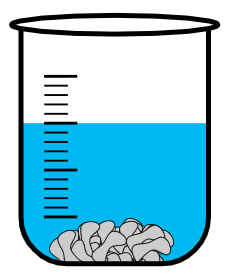
\includegraphics[scale=0.25]{images/sol cu metal zn.png} 
\end{center}
\end{minipage}%
\begin{minipage}{0.8\textwidth}
La réaction a-t-elle lieu ? $\Box$ oui $\Box$ non \\[2mm]
Écrire les deux demi équations correspondantes à cette réaction. \\[2mm]
\LARGE{\fbox{$~~~~~~~~ ~~ \longrightarrow~~~~~~~~+ ~~~~~~~~$} ~~~~~~~~ \fbox{$~~~~~~~~+ ~~~~~~~~ \longrightarrow ~~~~~~ $}}\\[2mm]
\normalsize
Écrire l'équation de la réaction. \\[2mm]
\fbox{\LARGE {$~~~~~~~~~~+ ~~~~~~~~~~ \longrightarrow~~~~~~~~~~+ ~~~~~~~~ $}}\\

\end{minipage}
\end{figure}

\vspace {5mm}

\textbf{Exp~~\ding{203} :} On introduit des tournures de cuivre dans une solution contenant des ions \ch{Zn\pch[2]}
\begin{figure}[h]
\begin{minipage}{0.7\textwidth}
La réaction a-t-elle lieu ? $\Box$ oui $\Box$ non \\[2mm]
Écrire les deux demi équations correspondantes à cette réaction. \\[2mm]
\LARGE{\fbox{$~~~~~~~~ ~~ \longrightarrow~~~~~~~~+ ~~~~~~~~$} ~~~~~~~~ \fbox{$~~~~~~~~+ ~~~~~~~~ \longrightarrow ~~~~~~ $}}\\[2mm]
\normalsize
Écrire l'équation de la réaction. \\[2mm]
\fbox{\LARGE {$~~~~~~~~~~+ ~~~~~~~~~~ \longrightarrow~~~~~~~~~~+ ~~~~~~~~ $}}\\

\end{minipage}
\begin{minipage}{0.3\textwidth}
\begin{center}
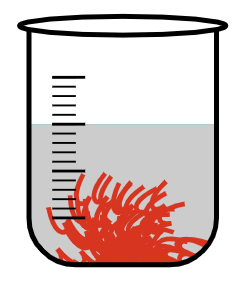
\includegraphics[scale=0.25]{images/sol zn metal cu.png} 
\end{center}
\end{minipage}%
\end{figure}

\vspace {5mm}

\textbf{Exp~~\ding{204} :} On introduit des clous en fer dans une solution contenant des ions \ch{Ag\pch[]}
\begin{figure}[h]
\begin{minipage}{0.3\textwidth}
\begin{center}
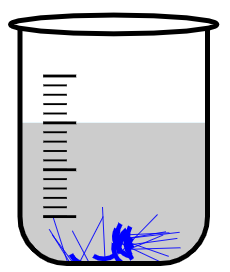
\includegraphics[scale=0.25]{images/sol Al metal Fe.png} 
\end{center}
\end{minipage}%
\begin{minipage}{0.8\textwidth}
La réaction a-t-elle lieu ? $\Box$ oui $\Box$ non \\[2mm]
Écrire les deux demi équations correspondantes à cette réaction. \\[2mm]
\LARGE{\fbox{$~~~~~~~~ ~~ \longrightarrow~~~~~~~~+ ~~~~~~~~$} ~~~~~~~~ \fbox{$~~~~~~~~+ ~~~~~~~~ \longrightarrow ~~~~~~ $}}\\[2mm]
\normalsize
Écrire l'équation de la réaction. \\[2mm]
\fbox{\LARGE {$~~~~~~~~~~+ ~~~~~~~~~~ \longrightarrow~~~~~~~~~~+ ~~~~~~~~ $}}\\

\end{minipage}
\end{figure}

\vspace {5mm}

\textbf{Exp~~\ding{205} :} On introduit de la grenaille de zinc dans une solution contenant des ions \ch{Fe\pch[2]}
\begin{figure}[h!]
\begin{minipage}{0.7\textwidth}
La réaction a-t-elle lieu ? $\Box$ oui $\Box$ non \\[2mm]
Écrire les deux demi équations correspondantes à cette réaction. \\[2mm]
\LARGE{\fbox{$~~~~~~~~ ~~ \longrightarrow~~~~~~~~+ ~~~~~~~~$} ~~~~~~~~ \fbox{$~~~~~~~~+ ~~~~~~~~ \longrightarrow ~~~~~~ $}}\\[2mm]
\normalsize
Écrire l'équation de la réaction. \\[2mm]
\fbox{\LARGE {$~~~~~~~~~~+ ~~~~~~~~~~ \longrightarrow~~~~~~~~~~+ ~~~~~~~~ $}}\\

\end{minipage}
\begin{minipage}{0.3\textwidth}
\begin{center}
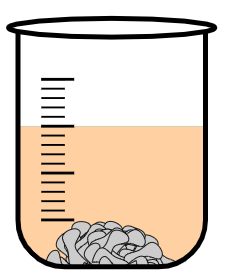
\includegraphics[scale=0.25]{images/sol fer metal zinc.png} 
\end{center}
\end{minipage}%
\end{figure}

\newpage

\textbf{Exp~~\ding{206} :} On introduit des clous en fer dans une solution contenant des ions \ch{Al\pch[3]}
\begin{figure}[h]
\begin{minipage}{0.3\textwidth}
\begin{center}
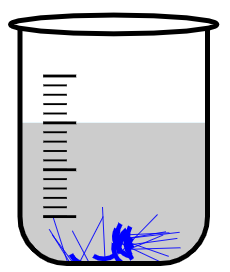
\includegraphics[scale=0.25]{images/sol Al metal Fe.png} 
\end{center}
\end{minipage}%
\begin{minipage}{0.7\textwidth}
La réaction a-t-elle lieu ? $\Box$ oui $\Box$ non \\[2mm]
Écrire les deux demi équations correspondantes à cette réaction. \\[2mm]
\LARGE{\fbox{$~~~~~~~~ ~~ \longrightarrow~~~~~~~~+ ~~~~~~~~$} ~~~~~~~~ \fbox{$~~~~~~~~+ ~~~~~~~~ \longrightarrow ~~~~~~ $}}\\[2mm]
\normalsize
Écrire l'équation de la réaction. \\[2mm]
\fbox{\LARGE {$~~~~~~~~~~+ ~~~~~~~~~~ \longrightarrow~~~~~~~~~~+ ~~~~~~~~ $}}\\

\end{minipage}
\end{figure}



\textbf{Exp~~\ding{207} :} On introduit de la grenaille de chrome (Cr) dans une solution contenant des ions cuivre (\ch{Cu\pch[2]})

\begin{figure}[h]
\begin{minipage}{0.2\textwidth}
\begin{center}
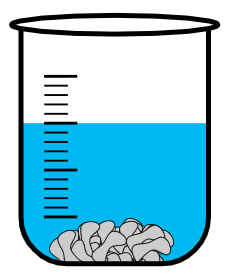
\includegraphics[scale=0.25]{images/sol cu metal zn.png} 
\end{center}
\end{minipage}%
\begin{minipage}{0.8\textwidth}
La réaction a-t-elle lieu ? $\Box$ oui $\Box$ non \\[2mm]
Écrire les deux demi équations correspondantes à cette réaction. \\[2mm]
\LARGE{\fbox{$~~~~~~~~ ~~ \longrightarrow~~~~~~~~+ ~~~~~~~~$} ~~~~~~~~ \fbox{$~~~~~~~~+ ~~~~~~~~ \longrightarrow ~~~~~~ $}}\\[2mm]
\normalsize
Écrire l'équation de la réaction. \\[2mm]
\fbox{\LARGE {$~~~~~~~~~~+ ~~~~~~~~~~ \longrightarrow~~~~~~~~~~+ ~~~~~~~~ $}}\\

\end{minipage}
\end{figure}

\vspace {5mm}

\textbf{Exp~~\ding{208} :} On introduit des morceau de Magnésium (Mg) dans une solution contenant des ions Nickel (\ch{Ni\pch[2]})
\begin{figure}[h]
\begin{minipage}{0.7\textwidth}
La réaction a-t-elle lieu ? $\Box$ oui $\Box$ non \\[2mm]
Écrire les deux demi équations correspondantes à cette réaction. \\[2mm]
\LARGE{\fbox{$~~~~~~~~ ~~ \longrightarrow~~~~~~~~+ ~~~~~~~~$} ~~~~~~~~ \fbox{$~~~~~~~~+ ~~~~~~~~ \longrightarrow ~~~~~~ $}}\\[2mm]
\normalsize
Écrire l'équation de la réaction. \\[2mm]
\fbox{\LARGE {$~~~~~~~~~~+ ~~~~~~~~~~ \longrightarrow~~~~~~~~~~+ ~~~~~~~~ $}}\\

\end{minipage}
\begin{minipage}{0.3\textwidth}

\begin{center}
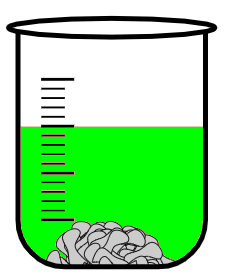
\includegraphics[scale=0.25]{images/sol nickel metal mg.png} 
\end{center}
\end{minipage}%
\end{figure}

\dotfill

\begin{center}
\large {ANNEXE - Classification des couples redox}

\dotfill 


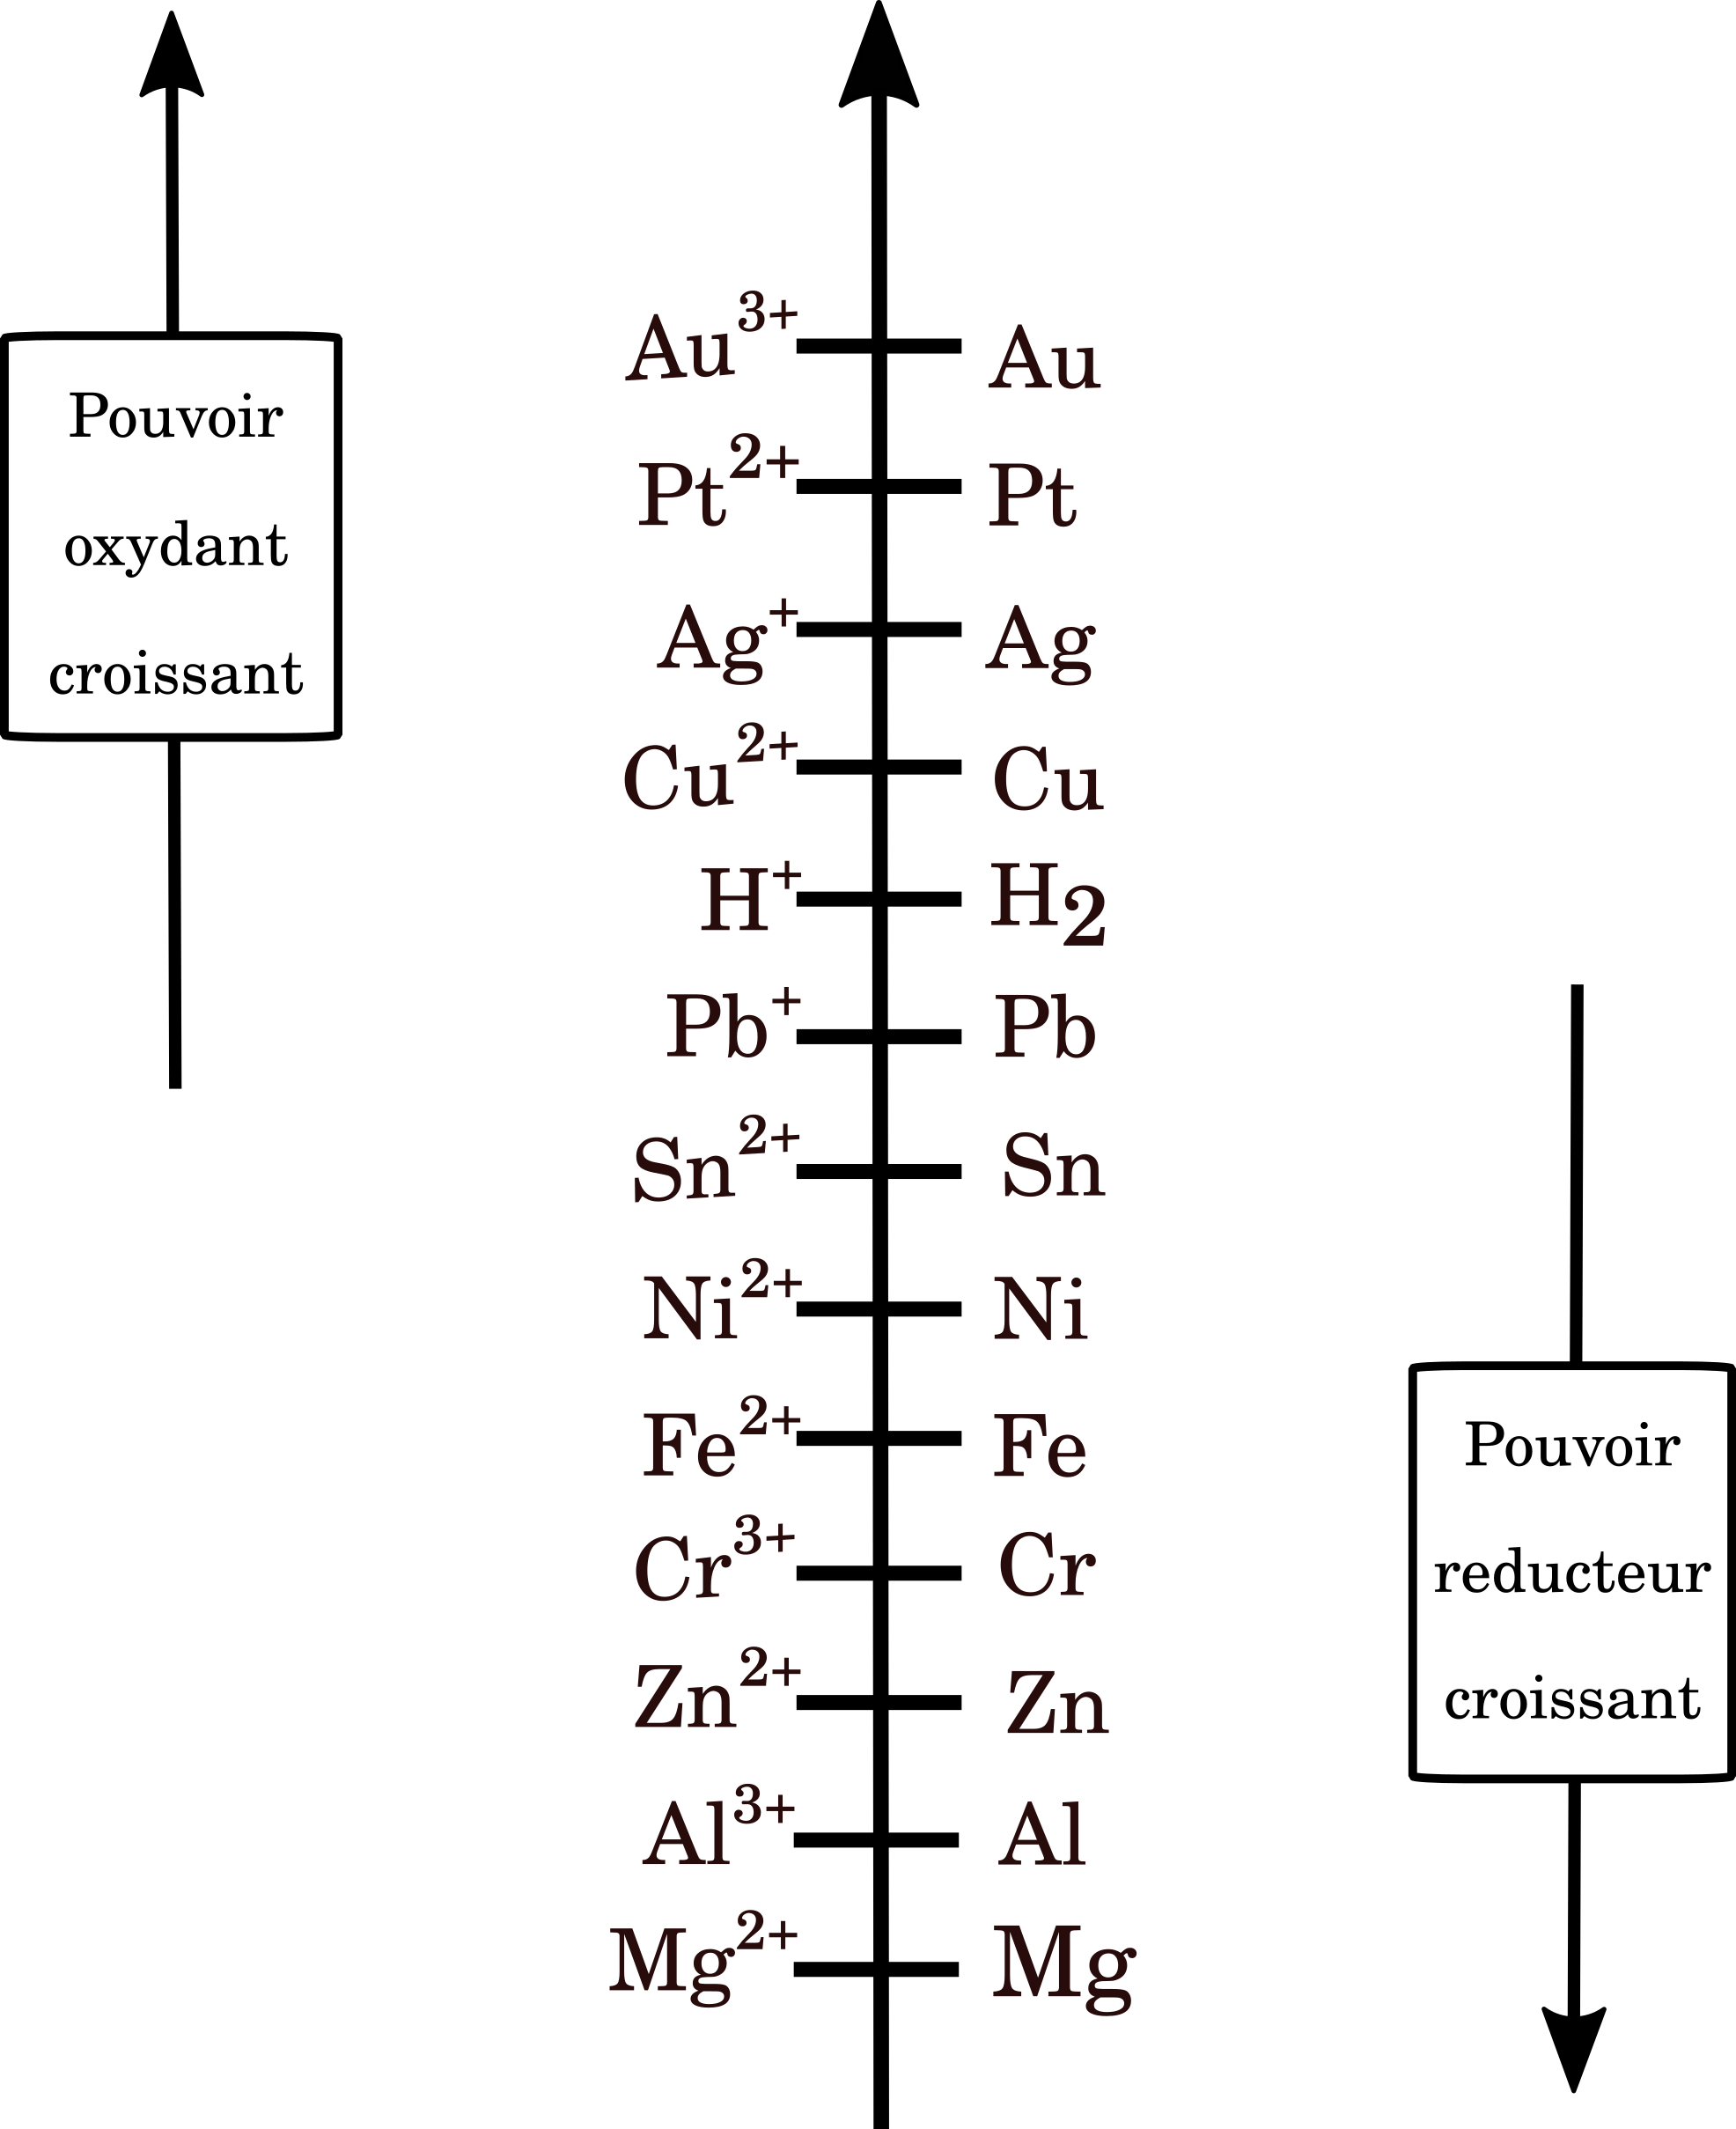
\includegraphics[scale=0.35]{images/classification.png} 
\end{center}
\vfill



\textbf{Exercice 2 : QCM}~~Parmi les trois propositions, choisissez la bonne réponse. 
\begin{center}
\renewcommand{\arraystretch}{2.5}
\begin{tabular}{|m{4mm}|p{4.5cm}||m{3.5cm}|m{3.5cm}|m{3.5cm}|}
    \hline
    \ding{202} & Au cours d'une réaction d'oxydo-réduction, il se produit un transfert  & de protons & de neutrons & d'électrons \\
    \hline
    
    \ding{203} & Dans quel cas l'ion en solution ne se dépose-t-il pas sur la lame métallique  & ~~~~~~~~\raisebox{-.7\height}{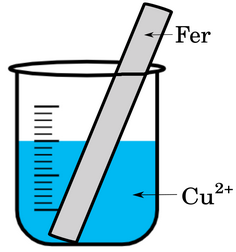
\includegraphics[scale=1]{images/QCm1.png}}& ~~~~~~~~\raisebox{-.7\height}{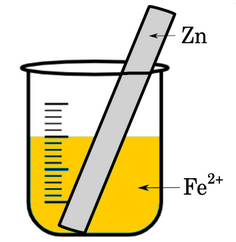
\includegraphics[scale=1.05]{images/QCm2.png}} & ~~~~~~~~\raisebox{-.7\height}{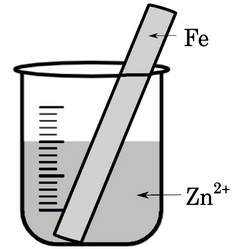
\includegraphics[scale=1]{images/QCm3.png}} \\
    \hline
    \ding{204} & Une oxydation est   & une perte d'électrons & un gain d'électrons & une perte de protons \\
    \hline
    \ding{205} & Au cours d'une réaction chimique l'étain (\ch{Sn}) se transforme en ions étain II (\ch{Sn\pch[2]}), on dit  & qu'il se réduit  & qu'il se protège & qu'il s'oxyde \\
    \hline
    \ding{206} & Par quelle équation peut-on traduire l'oxydation de l'aluminium &  $$\ch{Al\pch[3]} \longrightarrow \ch{Al}+ 3\ch{e\mch[]}$$ & $$\ch{Al} \longrightarrow \ch{Al\mch[3]}+ 3\ch{e\mch[]}$$& $$\ch{Al} \longrightarrow \ch{Al\pch[3]}+ 3\ch{e\mch[]}$$ \\
    \hline
    \ding{207} & Le zinc est plus réducteur que le plomb qu'elle est l'équation de réduction possible &  \small{$$2\ch{Pb\pch[]}+ \ch{Zn\pch[2]}\longrightarrow 2\ch{Pb}+ \ch{Zn}$$ }
    & 
    \small{$$2\ch{Pb} + \ch{Zn\pch[2]}\longrightarrow \ch{Zn}+ 2\ch{Pb\pch[ ]}$$}
    & 
    \small{$$\ch{Zn}+ 2\ch{Pb\pch[]}\longrightarrow 2\ch{Pb} + \ch{Zn\pch[2]}$$} \\
    
    \hline
    \ding{208} & Que faut-il faire pour écrire l'équation bilan de ~~~~~~~~ $ \ch{Al}\longrightarrow \ch{Al\pch[3]}+ 3\ch{e\mch[]}$ et $ \ch{Ag \pch[]}+\ch{e\mch[]}\longrightarrow \ch{Ag}$  & additionner membres à membres  &  multiplier par 3 la première demi-équation puis additionner membre à membre & multiplier par 3 la seconde demi-équation puis additionner membre à membre \\
    \hline
   
\end{tabular}

\end{center}

\newpage


\end{document}